\documentclass[a4paper,12pt]{article}

\usepackage[T2A]{fontenc} 
\usepackage[utf8]{inputenc}
\usepackage[english,russian]{babel}
\usepackage{listings}
\usepackage[dvips]{graphicx}
\usepackage{indentfirst}
\usepackage{color}
\usepackage{hyperref}
\usepackage{amsmath}
\usepackage{amssymb}
\usepackage{geometry}
\geometry{left=1.5cm}
\geometry{right=1.5cm}
\geometry{top=1cm}
\geometry{bottom=2cm}

\graphicspath{{images/}}

\begin{document}
\sloppy

\lstset{
	basicstyle=\small,
	stringstyle=\ttfamily,
	showstringspaces=false,
	columns=fixed,
	breaklines=true,
	numbers=right,
	numberstyle=\tiny
}

\newtheorem{Def}{Определение}[section]
\newtheorem{Th}{Теорема}
\newtheorem{Lem}[Th]{Лемма}
\newenvironment{Proof}
	{\par\noindent{\bf Доказательство.}}
	{\hfill$\scriptstyle\blacksquare$}
\newenvironment{Solution}
	{\par\noindent{\bf Решение.}}
	{\hfill$\scriptstyle\blacksquare$}


\begin{flushright}
	Кринкин М. Ю. группа 504 (SE)
\end{flushright}

\section{Домашнее задание 8}

\paragraph{Задание 1.} Доказать, что число Каталана $c_n$ равно:
\begin{enumerate}
\item количеству способов разбиения выпуклого $(n+2)$ - уголтника на треугольники диагоналями, не пересекающимися внутри многоугольника;

\item количеству способов соединения $2n$ точек на окружности $n$ непересекающимися отрезками;

\item количеству монотонных отображений из $n$-множества $\left[n\right] = \{1, 2, ..., n\}$ в $\left[n\right]$, таких, что $f\left(i\right) \le i$ для любого $i \in \left[n\right]$;

\item количеству двоичных деревьев (из любой вершины выходит не более двух ребер) c $n$ вершинами;

\item количеству плоских деревьев с $\left(n+1\right)$ вершшинами;

\item количеству перестановок $a_1a_2...a_n$ множества $\left[n\right]$, которые можно упорядочить по возрастанию с помощью единственного стека.
\end{enumerate}

\begin{Solution}
Пронумеруем все вершины от $1$ до $n+2$. Каждый треугольник будет опираться на некоторую сторону $(i, i+1)$, более того на эту сторону будет опираться только один треугольник. Рассмотрим сторону $(n+1, n+2)$ количество способов добавить к стороне вершину, так чтобы получился треугольник равно количеству возможных вершин $n$ - штук.

\begin{figure}[h]
\center{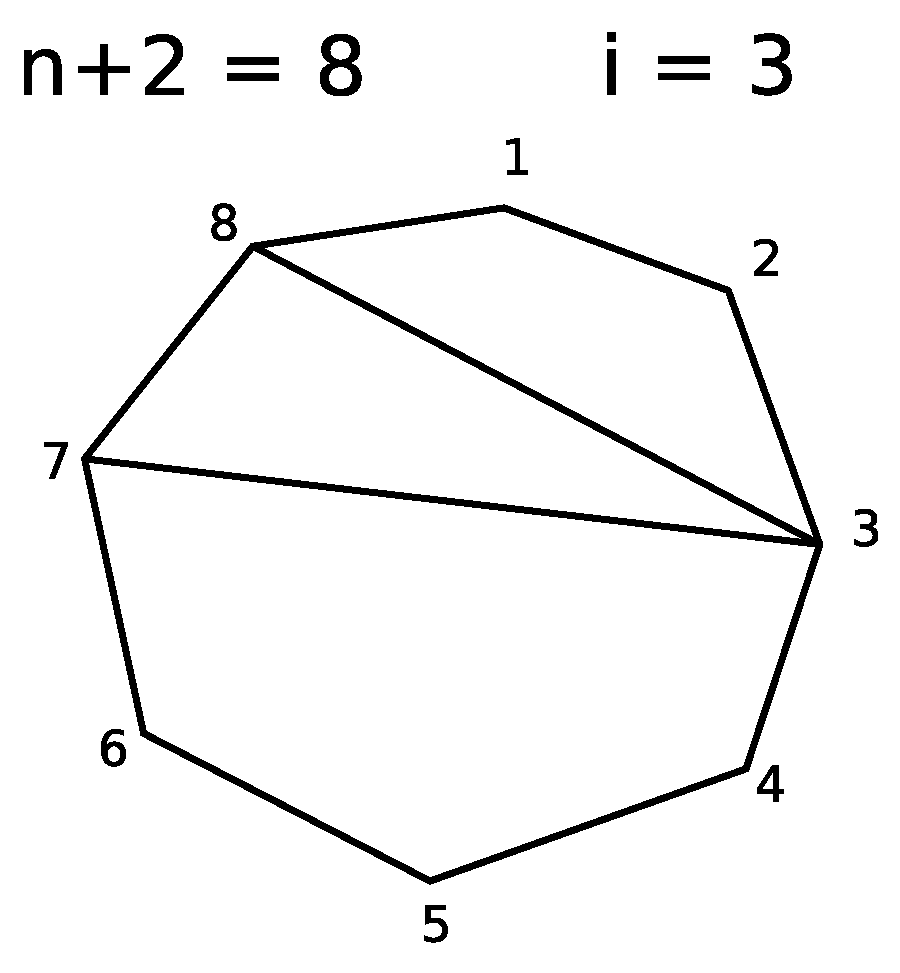
\includegraphics[width=0.2\linewidth]{simplex}}
\caption{Пример выбора опорной вершины и разбиения многоугольника}
\label{img::simplex}
\end{figure}

Пусть мы выбрали эту вершину и это вершина $i$ (см. рисунок \ref{img::simplex}). Тогда после <<вырезания>> треугольника получаем два многоугольника с количеством вершин $i+1$ и $n + 2 - i$ (т. е. вершина $i$ продублировалась в оба многоугольника, а $n+1$ и $n+2$ поделились между ними). Разбить первый из них можно $c_{i-1}$ способами, а второй $c_{n-i}$. Продолжаем процесс для каждого вновь образовонного многоугольника, пока не получим треугольник.

$i$ принимает значения от $1$ до $n$, число способов триангуляции для выбранной вершины $i$ равно $c_{i-1} c_{n-i}$, суммируем по всем $i$:
\[
	c_{n} = c_0 c_{n-1} + c_1 c_{n-2} + ... + c_{n-1} c_0
\]
теперь осталось проверить только начальные условия, которые очевидно выполняются.

Рассмотрим вторую задачу. Пусть у нас $2n$ точек расставлено на окружности. Выбрем в нем начальную вершину пусть она имеет номер $1$. Соединить эту вершину можно только так, чтобы слева и справа от проведенного ребра оставалось четное количество точек, таким образом можно соединить вершину $1$ только с вершинами $2i$, где $i \in \overline{1,n}$ (с вершиной имеющей четный номер). После проведения отрезка $(1, 2i)$ наша задача распадается на две подзадачи, решение, которых эквивалентно решению исходной задачи меньшей размерности. Справа от $(1, 2i)$ остается $2i - 2 = 2(i-1)$ точек, а слева $2n - 2i + 2 = 2(n-i+1)$. Таким образом, если для $2k$ точек решением является число $c_k$, то $c_n = \sum_{i=1}^n c_{i-1} c_{n-i+1} = \sum_{i=0}^{n-1} c_i c_{n-i}$. Остается проверить лишь начальные условия.

Можно показать, что эта задача эквивалентна задаче о скобочных последовательностях. Каждая вершина $i$ от 1 до $2n$ соответствует $i$-ой позиции в строке скобок, причем, если вершина соединена с вершиной меньшего номера, то она соответствует закрывающей скобке, иначе вершина соответствует открывающей скобке. Очевидно, что такие пары соответствуют правильным скобочным последовательностям, и каждой скобочной последовательности спосотавляется $2n$ точек соединенных $n$ отрезками.

Строим двудольный граф отображения. Вершины первой доли - элементы из проецируемого множества, а вершины второй доли - элементы множества, на которое происходит отображение. Вершина из первой доли связана ребром с вершиной из второй доли, если элемент соответствующий вершине первой доли переходит в элемент соответствующий вершине второй доли. Пример графов для оторбажения из $\left[3\right]$ в $\left[3\right]$ приведен на рисунке \ref{img::mapping}.

\begin{figure}[h]
\center{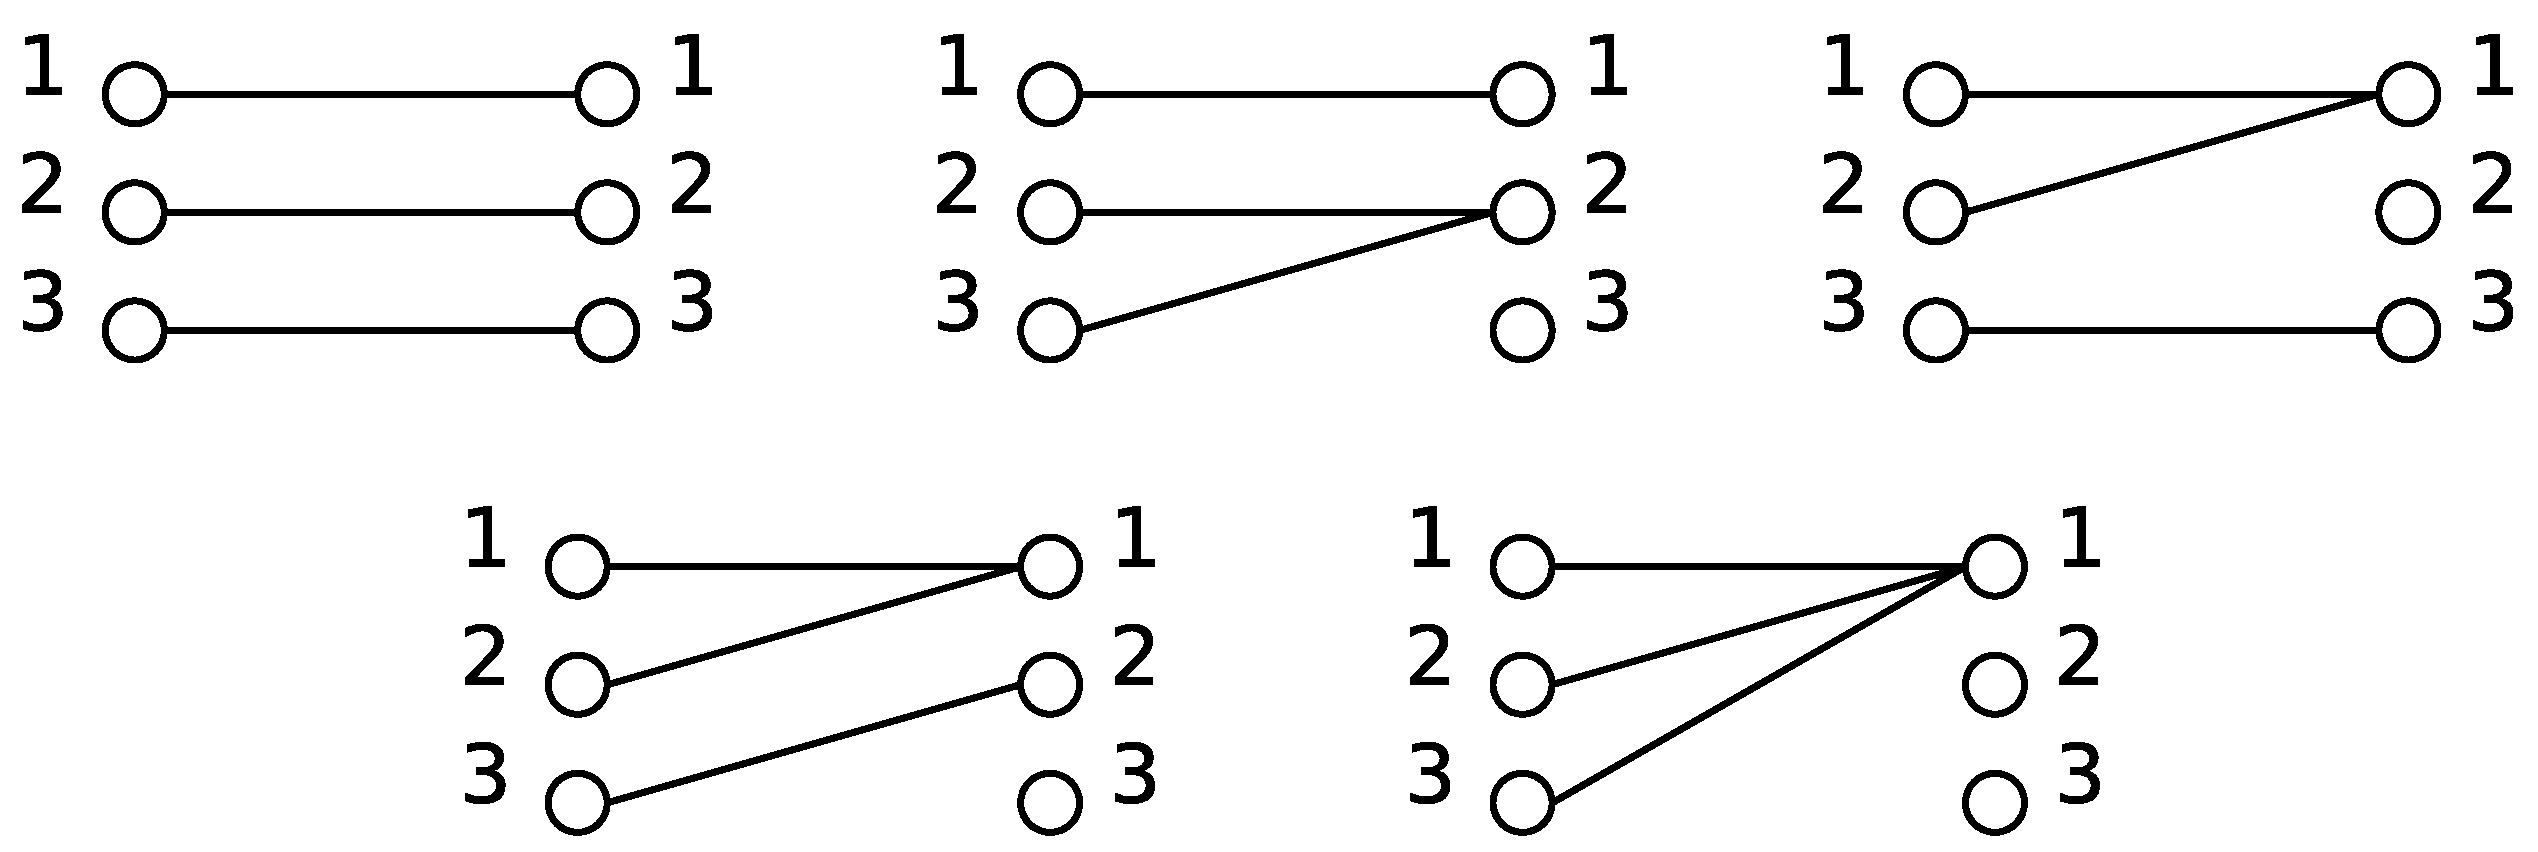
\includegraphics[width=0.3\linewidth]{mapping}}
\caption{Графы отображений}
\label{img::mapping}
\end{figure}

Каждому такому графу можно сопоставить путь на плоскости (см. рисунок \ref{img::paths}). На рисунке, на вертикали соответствующей $i$-ой вершине присутсвует стрелка вверх длины $k$, где $k$ - степень вершины $i$ из второй доли.

\begin{figure}[h]
\center{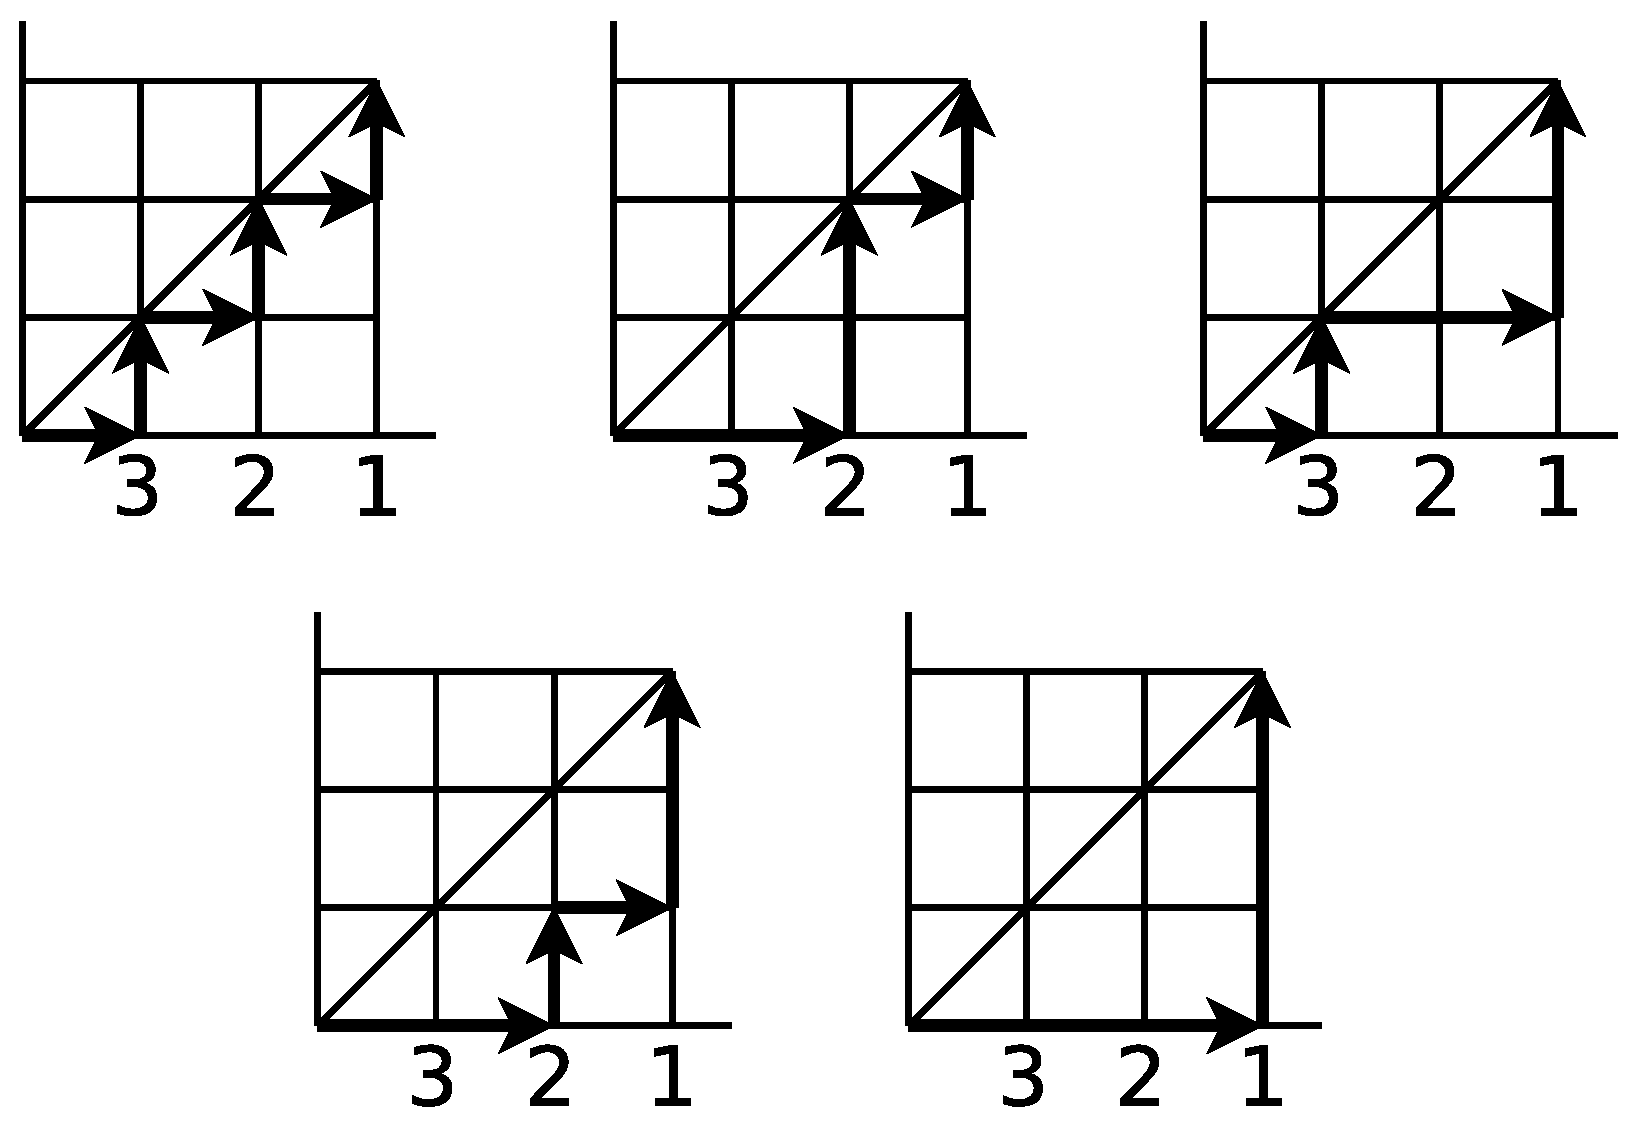
\includegraphics[width=0.3\linewidth]{paths}}
\caption{Пути на плоскости, соответствующие графам отображений}
\label{img::paths}
\end{figure}

Эти пути аналогичны путям Дика, и их количество также определяется числами Каталана. Но можно свести задачу и к задаче о скобочных последовательностях: шаг на единицу вправо - одна открывающая скобка, шаг на единицу вверх - закрывающая.

Двоичное дерево - корень и два двоичных поддерева (возможно пустых) - левое и правое. Построим корень, остается $n-1$ вершина. Мощность левого и правого поддерва изменяется от $0$ до $n-1$ причем, если $n_l$ - мощность левого поддерва, а $n_r$ - мощность правого, то $n_l + n_r = n-1$. Теперь, если $bt_n$ - число двоичных деревьев из $n$ вершин, то для нее справедлива рекуррентная формула:
\[
	bt_n = \sum_{i=0}^{n-1} bt_i bt_{n-1-i}
\]
начальные условия проверяются просто и совпадают с начальными условия для чисел Каталана, т. е. получаем ту же самую последовательность.

В пятой задаче поступим следующим образом. Будем обходть дерево из некоторого корня пока не вернемся опять в корень. Если мы проходим по ребру нечетный раз (1, 3, 5 ...) то пишем открывающую скобку, иначе закрывающую. Таким образом получим, очевидно, только правильную скобочную последовательность.

В дереве $n-1$ ребер, пройти все ребра из некоторого корня и вернуться назад можно пройдя по каждому ребру ровно два раза, по такому обходу можно построить правильную скобочную последовательность из $2n$ скобок (по каждому ребру 2 раза).

Правда тут стоит заметить, что может существовать несколько таких обходов дерева, соответствующих разным скобочным последовательностям, но по каждой скобочной последовательности дерево восстанавливается однозначно, т. е. каждой скобочной последовательности мы можем сопоставить свое собственное дерево (если например восстанавливая дерево по скобочной последовательности нумеровать все ребра см. рис \ref{img::treetrav}).

Так как количество скобочных последовательностей определяется числами каталана, то и количество соответствующих им деревьев также определяется числами каталана. На рисунке \ref{img::treetrav} показано, как восстанавливать по скобочной последовательности дерево (и наоборот, как по дереву строить скобочную последовательность).

\begin{figure}[h]
\center{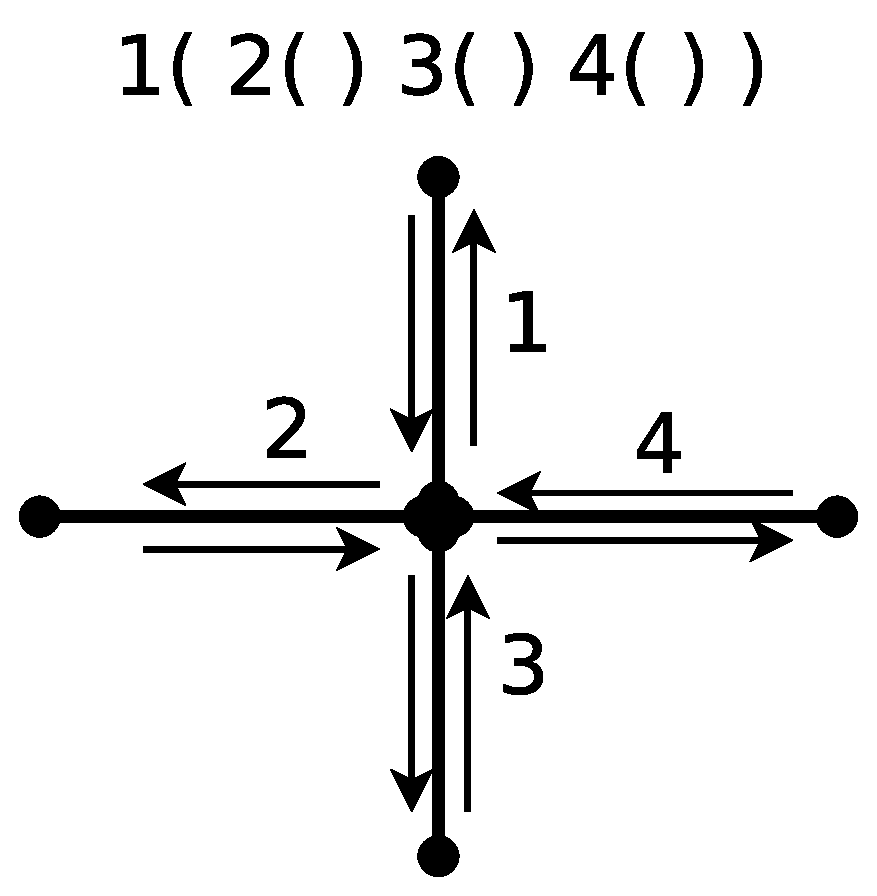
\includegraphics[width=0.3\linewidth]{treetrav}}
\caption{Соответствие деревьев и скобочных последовательностей}
\label{img::treetrav}
\end{figure}

Теперь покажем это же более формально. Очевидно, что число сопсобов построить дерево из 2 вершин $t_{1+1} = 1$ и из 1 вершины $t_{0+1} = 1$. Строим теперь все деревья из $n+1$ вершины, где $n \not= 0$. Строим ребро $(v_1, v_2)$, вершины от вершин $v_1$ и $v_2$ можно построить дерево (построить дерево от вершины $v_1$ - построить дерево с вершиной $v_1$, не включающее уже использованные вершины и построенные ребра). Количество вершин в деревьях построенных от $v_1$ или $v_2$ от $1 до n$, если не считать $v_1$ и $v_2$, то получаем диапазон $\overline{0, n-1}$. продолжая процесс рекурсивно построим дерево включающее все $n+1$ вершин.  Суммируя по всем мощностям деревьев построенных от вершин $v_1$ и $v_2$ получаем рекуррентное соотношение:
\[
	t_{n+1} = \sum_{i=0}^{n-1} t_{i+1} t_{n-1-i+1}
\]
Уравнение соответствует уравнению для чисел Каталана с точностью до индексации и начальные условия выполняются, следовательно числа совпадают.

Наконец последнаяя задача, проходя последовательность элементов поочередно слева направо и занося (или не занося) элементы в стек осортировать ее можно только если последоваетльность $seq = seq_1 a_n seq_2$ удовлетворяет условию, что все элементы $seq_1$ меньше или равны всем элементам $seq_2$, потому что в противном случае нам бы пришлось занести $seq_1 n$ в стек, но так как $n$ - наибольшее число последовательности, то оно должно попасть в самый низ стека, что не получается, с дургой стороны, если условие выполняется, то можно отсортировать $seq_1$ после чего стек освободится, далее мы заносим в него $n$ и сортируем $seq_2$, после чего достаем из стека $n$. Каждая из подпоследовательностей $seq_1$ и $seq_2$ должны опятьже удовлетворять условию, чтобы их можно было отсортировать таким образом.

Рекуррентное соотношение составляется суммируованием по позиции максимального элемента $n$, он может распологаться на $n$ позициях с $1$ до $n$, тогда:
\[
	S_n = \sum_{i=1}^{n} S_{i-1} S_{n-i} = \sum_{i=0}^{n-1} S_{i} S_{n-1-i}
\]
т. е получаем рекуррентное соотношение для чисел Каталана, начльные условия легко проверяются.
\end{Solution}


\paragraph{Здание 2.} Числом Моцкина $M_n$ называется число решоточных путей из точки $(0,0)$ в точку $(0,n)$, не опускающихся ниже оси $y=0$ и составленных из шагов $(1,0)$, $(1,1)$ и $(1,-1)$. Найти для этих чисел рекуррентное соотношение и обыкновенную производящую функцию.

\begin{Solution}
Закодируем каждый путь Моцкина некоторым словом, вектору $\left(1,1\right)$ сопоставим открывающую скобку, вектору $\left(1,-1\right)$ сопоставим закрывающую скобку, а $\left(1, 0\right)$ - букву $x$. Если слово начинается с $x$, то <<отрезав>> $x$ опять получаем слово Моцкина, но длины на единицу меньше, если же начинается с открывающей скобки, то находим соответствующую закрывающую скобку, т. е. имеем $\left(s_1\right)s_2$, $s_1$ и $s_2$ - правильные слова Моцкина, и если $\left|\left(s_1\right)s_2\right| = n$ и $\left|s_1\right| = i$, то $\left|s_2\right| = n-2-i$. Тогда просуммировав по всем $i = \overline{0,n-2}$, получаем рекуррентное соотношение:
\[
	m_{n+2} = m_{n+1} = \sum_{i=0}^n m_{n-i} m_i
\]
Теперь получим обыкновенную производящую функцию, пусть:
\[
	f\left(x\right) = m_0 + m_1 x + m_2 x^2 + m_3 x^3 + ...
\]
Домножим рекуррентное соотношение на $x^{n+2}$ и просуммируем по всем $n$:
\[
	\begin{split}
		& \sum_{n=0}^{\infty}m_{n+2} x^{n+2} = x \sum_{n=0}^{\infty} m_{n+1} x^{n+1} + x^2 \sum_{n=0}^{\infty} x^n \left[\sum_{i=0}^{n} m_{n-i} m_i\right] \Rightarrow \\
		& \Rightarrow f\left(x\right) - m_0 - m_1 = x \left(f\left(x\right) - m_0\right) + x^2 \left(f\left(x\right)\right)^2 \Rightarrow \\
		& \Rightarrow x^2 \left(f\left(x\right)\right)^2 + f\left(x\right)\left(x - 1\right) + m_0 + m_1 - x m_0 = 0\Rightarrow \\
		& \Rightarrow x^2 \left(f\left(x\right)\right)^2 + f\left(x\right)\left(x - 1\right) + 2 - x = 0 \\
		& f\left(x\right) = \frac{\left(1-x\right) - \sqrt{\left(1-x\right)^2 - 4x^2\left(2-x\right)}}{2x^2}
	\end{split}
\]
\end{Solution}

\paragraph{Задание 3.} Треугольник Дика перечисляет пути в положительном квадранте плоскости, выходящие из начала координат и составленные из векторов $(1,1)$ и $(1,-1)$. Найти для жтих чисел рекуррентное соотношение и производящую функцию вида:
\[
	f\left(t,x\right) = \sum_{n=0}^{\infty} \sum_{k=0}^n a_{n,k} x^k \frac{t^n}{n!}
\]

\begin{Solution}
Рекуррентное соотношение для чисел в узлах треугольника Дика:
\[
	a_{n,k} = a_{n-1, k-1} + a_{n-1,k+1}
\]
т. е. значение в точке $a_{n,k}$ определяется значениями в точках слева выше и слева ниже от нее.
Начальные условия для рекуррентного соотношения:
\[
	\begin{split}
		& a_{n,n} = 1 \\
		& a_{n,k} = 0, k > n \\
		& a_{n,k} = 0, k < 0
	\end{split}
\]
Далее немного схитрим, преобразуем треугольник Дика к следующему виду:
\[
	\begin{matrix}
		n \backslash k  & 0 & 1 & 2 & 3 & 4 \\
		0 & 1 \\
		1 & 1 & 1 \\
		2 & 1 & 2 & 2 \\
		3 & 1 & 3 & 5 & 5 \\
		4 & 1 & 4 & 9 & 14 & 14 \\
	\end{matrix}
\]
В преобразованном треугольнике Дика рекуррентное соотношение принимает вид:
\[
	d_{n+1,k+1} = d_{n, k+1} + d_{n+1, k}
\]
(элемент $(n,k)$ - сумма эелементов сверху и слева, т. е. каждая строка - диагональ исходного треугольника Дика)
Найдем двумерную экспоненциаьную функцию:
\[
	\begin{split}
		& d_{n+1, k+1} x^{k+1} = d_{n, k+1} x^{k+1} + x d_{n+1, k} x^k \Rightarrow \\
		& \Rightarrow \sum_{k=0}^{\infty} d_{n+1, k+1} x^{k+1} = \sum_{k=0}^{\infty} d_{n, k+1} x^{k+1} + x \sum_{k=0}^{\infty} d_{n+1, x} x^k \Rightarrow \\
		& \Rightarrow d_{n+1} - d_{n+1, 0} = d_{n} - d_{n, 0} + x d_{n+1} \Rightarrow d_{n+1} \left(1 - x\right) = d_{n} \Rightarrow \\
		& \Rightarrow \left(1 - x\right) \sum_{t = 0}^{\infty} d_{n+1} \frac{t^{n+1}}{\left(n+1\right)!} = \sum_{n=0}^{\infty} d_{n} \frac{t^{n+1}}{\left(n+1\right)!} \Rightarrow \\
		& \Rightarrow \left(1 - x\right)f'\left(t,x\right) = f\left(t,x\right) \Rightarrow f\left(t,x\right) = e^{\frac{t}{1-x}}
	\end{split}
\]
\end{Solution}

\paragraph{Задание 4.} Определить количество способов размещения $n$ гостей в трех комнатах при условии, что в первой комнате находится хотя бы 1 гость, нечетное число гостей находится во второй комнате, и четное - в третьей.

\begin{Solution}
Рассмотрим сначала случай, когда все гости неразличимы, то есть принципиально лишь количество гостей в каждой комнате. В этом случае используем обыкновенные производящие функции для последовательностей:
\[
	0, 1, 1, 1, 1, 1, 1, ...
\]
\[
	0, 1, 0, 1, 0, 1, 0, 1, ...
\]
\[
	1, 0, 1, 0, 1, 0, 1, 0, ...
\]
Для первой последовательности производящая функция уже хорошо известна:
\[
	f_1\left(x\right) = \frac{x}{1-x}
\]
Две оставшиеся можно найти из уравнения:
\[
	\begin{split}
		& x f_3\left(x\right) = f_2\left(x\right) \\
		& x f_3\left(x\right) + f_3\left(x\right) = \frac{1}{1 - x} \Rightarrow \\
		& \Rightarrow f_3\left(x\right) = \frac{1}{1 - x^2} \Rightarrow f_2\left(x\right) = \frac{x}{1 - x^2}
	\end{split}
\]
Перемножаем все вместе:
\[
	\begin{split}
		& r\left(x\right) = f_1\left(x\right) f_2\left(x\right) f_3\left(x\right) = \frac{x}{1 - x} \frac{1}{\left(1 + x\right)\left(1 - x\right)} \frac{x}{\left(1 + x\right)\left(1 - x\right)} = \\
		& = - \frac{1/16}{1 - x} - \frac{1/4}{\left(1 - x\right)^2} + \frac{1/4}{\left(1 - x\right)^3} - \frac{1/16}{1 + x} + \frac{1/8}{\left(1 + x\right)^2} = \\
		& = -\frac{1}{16}\sum_{i=0}^{\infty}x^i - \frac{1}{4}\sum_{i=0}^{\infty} \left(i+1\right) x^i + \frac{1}{4} \sum_{i=0}^{\infty} \frac{\left(i+1\right)\left(i+2\right)}{2} x^i - \frac{1}{16}\sum_{i=0}^{\infty} \left(-1\right)^i x^i + \frac{1}{8}\sum_{i=0}^{\infty}\left(-1\right)^i\left(i+1\right)x^i
	\end{split}
\]
Теперь пусть все гости различимы, в данном случае пойдем от противного, посмотрим как должно выглядеть решение (совсем не обязательно находить его точный вид, достаточно примерного выражения). Заполнение 3 различных комнат различными гостями так, чтобы в сумме количество гостей было равно $n$ определяется выражением:
\[
	\sum_{i, j >= 0} \frac{n!}{i! j! \left(n - i - j\right)!}
\]
на это выражение в результате еще наложаться некоторые огрничения, но по ней уже можно сказать, что она получается в результате произведения экспоненциальных производящих функций. Рассмотрим последовательности, производящии функции которых определяют результат:
\[
	0, 1, 1, 1, 1, 1, 1, 1, ...
\]
нетрудно дать такой последовательностии комбинаторную интерпритацию - все варианты заполнения первой комнаты, кроме пустого, возможны, для второй комнаты последовательность:
\[
	0, 1, 0, 1, 0, 1, 0, ...
\]
заполнение второй комнаты четным числом гостей не должно учитываться, и наконец третья последовательность:
\[
	1, 0, 1, 0, 1, 0, 1, 0, ...
\]
заполнение нечетным количеством гостей невозможно, получили те же самые последовательности, что и в первом случае (если, конечно, все правильно). Производящая функция для первой последовательности:
\[
	F_1\left(x\right) = e^x - 1
\]
Производящие функции для второй и третьей последовательности:
\[
	\begin{split}
		& F_2\left(x\right) = sh\left(x\right) \\
		& F_3\left(x\right) = ch\left(x\right)
	\end{split}
\]
Произведение производящих функций дает:
\[
	\begin{split}
		& R\left(x\right) = F_1\left(x\right) F_2\left(x\right) F_3\left(x\right) = \left(e^x - 1\right) sh\left(x\right) ch\left(x\right) = \\
		& = \frac{e^x - e^{-x}}{2} \frac{e^x + e^{-x}}{2} \left(e^x - 1\right) = \frac{1}{4} \left(e^{3x} - e^{2x} - e^{-x} + e^{-2x}\right) = \\
		& = \frac{1}{4} \left(\sum_{i=0}^{\infty} 3^i \frac{x^i}{i!} - \sum_{i=0}^{\infty} 2^i \frac{x^i}{i!} - \sum_{i=0}^{\infty} \left(-1\right)^i \frac{x^i}{i!} + \sum_{i=0}^{\infty} \left(-2\right)^i \frac{x^i}{i!}\right)
	\end{split}
\]
\end{Solution}

\paragraph{Задание 5.} Определить количество чисел, состоящих из $n$ цифр, таких, что все цифры нечетные, а цифры 1 и 3 присутствуют в числе не менее 1 раза.

\begin{Solution}
Решим задачу сначала через экспоненциальные производящие функции. Последовательности соответствующие цифрам 5, 7, 9:
\[
	1, 1, 1, 1, 1, 1, ...
\]
последовательность соответствующая цифрам 1 и 3:
\[
	0, 1, 1, 1, 1, 1, ...
\]
Первой последовательности соответствует производящая функция:
\[
	e^x
\]
а второй:
\[
	e^x - 1
\]
Тогда производящая функция для результирующей последовательности:
\[
	\begin{split}
		& e^{3x} \left(e^x-1\right)^2 = e^{5x} - 2 e^{4x} + e^{3x} = \\
		& \sum_{i=0}^{\infty} 5^i \frac{x^i}{i!} - 2 \sum_{i=0}^{\infty} 4^i \frac{x^i}{i!} + \sum_{i=0}^{\infty} 3^i \frac{x^i}{i!}
	\end{split}
\]
Теперь найдем другое решение (более комбинаторное). Всего способов составить из 5 нечетных цифр $n$-значное число равно $5^n$, из них нам не подходят варианты, когда среди $n$ цифр отсутствует 1 или 3, т. е. получаем $5^n - 2 4^n$, теперь заметим, что числа в которых отсутствует и 1 и 3 были учтены 2 раза, следовательно окончательный результат $5^n - 2 \cdot 4^n + 3^n$
\end{Solution}

\paragraph{Задание 6.} Пусть каждый из $n$ различных телефонных столбов окрашен в один из следующих цветов: красный, белый, синий или желтый, причем число синих столбов нечетно, а число желтых четно. Сколькими способами это можно сделать?

\begin{Solution}
Данная задача эквивалентна случаю различных гостей в задаче 4 (представим, что гость окрашивается цветом комнаты, хотя это и не очень гуманно). Для красных и белых столбов последовательность следующая:
\[
	1, 1, 1, 1, 1, 1, 1, ...
\]
Каждое количество стобов возможно.
Для синих столбов последовательность следующая:
\[
	0, 1, 0, 1, 0, 1, 0, 1, 0, 1, ...
\]
а для желтых столбов:
\[
	1, 0, 1, 0, 1, 0, 1, 0, 1, 0, ...
\]
Производящие функции следующие:
\[
	\begin{split}
		& F_1\left(x\right) = e^x \\
		& F_2\left(x\right) = sh\left(x\right) \\
		& F_3\left(x\right) = ch\left(x\right)
	\end{split}
\]
Результат определяется произведением:
\[
	\begin{split}
		& R\left(x\right) = e^{2x}sh\left(x\right)ch\left(x\right) = e^{2x} \frac{e^x - e^{-x}}{2} \frac{e^x + e^{-x}}{2} = \\
		& = \frac{1}{4} \left(e^{4x} - 1\right) = \frac{1}{4}\left(e^{4x} - 1\right) = \frac{1}{4} \left(\sum_{i=0}^{\infty}4^i \frac{x^i}{i!} - 1\right)
	\end{split}
\]
\end{Solution}

\paragraph{Задание 7.} Предположим, что в предыдущей задаче используются оранжевый и зеленый цвета, причем число оранжевых, плюч число зеленых четно. Сколько теперь существует способов окрасить эти столбы?

\begin{Solution}
Задача сводится к нахождению производящей функции для последовательности:
\[
	1, 0, 2^2, 0, 2^4, 0, 2^6, 0, 2^8, 0, ...
\]
Но подобной производящей функцией мы уже пользовались выше:
\[
	F\left(x\right) = ch\left(2x\right)
\]
Домножаем полученный в предыдущей задаче результат на производящую функцию:
\[
	\begin{split}
		& R\left(x\right) = \frac{1}{4} \left(e^{4x} - 1\right) ch\left(2x\right) = \frac{1}{4} \left(e^{4x} - 1\right) \frac{e^x + e^{-x}}{2} = \\
		& = \frac{1}{8} \left(e^{5x} + e^{3x} - e^x - e^{-x}\right) = \frac{1}{8} \left(\sum_{i=0}^{\infty} 5^i \frac{x^i}{i!} + \sum_{i=0}^{\infty} 3^i \frac{x^i}{i!} - \sum_{i=0}^{\infty} \frac{x^i}{i!} - \sum_{i=0}^{\infty} \left(-1\right)^i \frac{x^i}{i!}\right)
	\end{split}
\]
\end{Solution}
\end{document}
